\chapter{\uppercase{System Design}} % Main chapter title
\label{ch:chap3} % For referencing

The focus of this chapter is to discuss the system architecture and various modules involved in the project. The modules used are listed below:

\begin{itemize}
    \item Course Recommendation
    \item Job Skillset Recommendation
    \item Chatbot Application
    \item Database Management
    \item Web Crawler
\end{itemize}

\section{System Architecture}
The architecture of the proposed system in Figure \ref{fig:system_architecture} comprises various modules, including the Course Recommendation Module, Job Skillset Recommendation Module, Chatbot Application Module, Database Management Module, and Web Crawler Module. These modules interact with each other to provide efficient course and job skillset recommendations to users.

\begin{figure}[h]
\centering
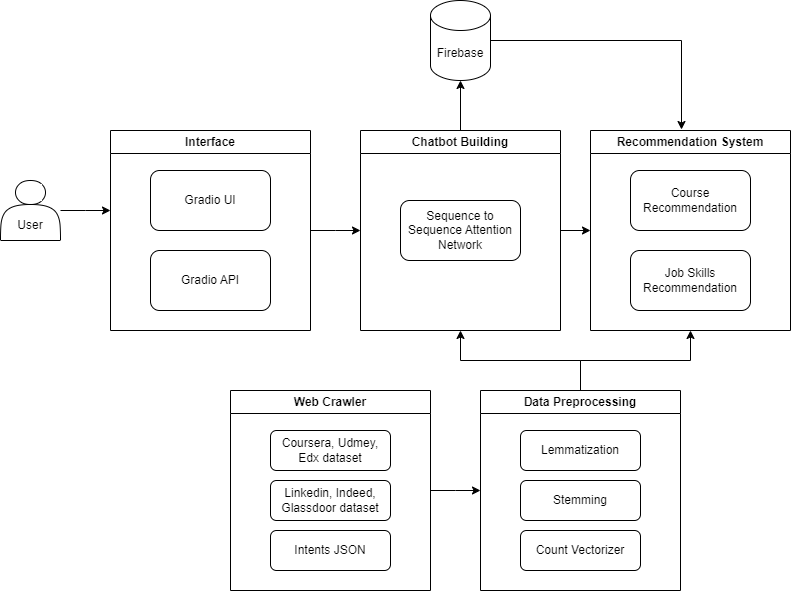
\includegraphics[width=0.8\textwidth]{3/system.png}
\caption{System Architecture}
\label{fig:system_architecture}
\end{figure}

\section{Input Data}

The input data consists of a dataset containing information about available courses and job skillsets, including attributes such as course titles, descriptions, prerequisites, and required skills.

\section{Preprocessing}

The preprocessing step involves cleaning and formatting the input data to prepare it for analysis. This may include removing duplicate entries, handling missing values, and standardizing the format of text fields.

\section{Chatbot Application}

The Chatbot Application Module provides a conversational interface for users to interact with the recommendation system. Users can input their preferences, career goals, and queries, and the chatbot responds with personalized course and job skillset recommendations.

\begin{figure}[h]
\centering
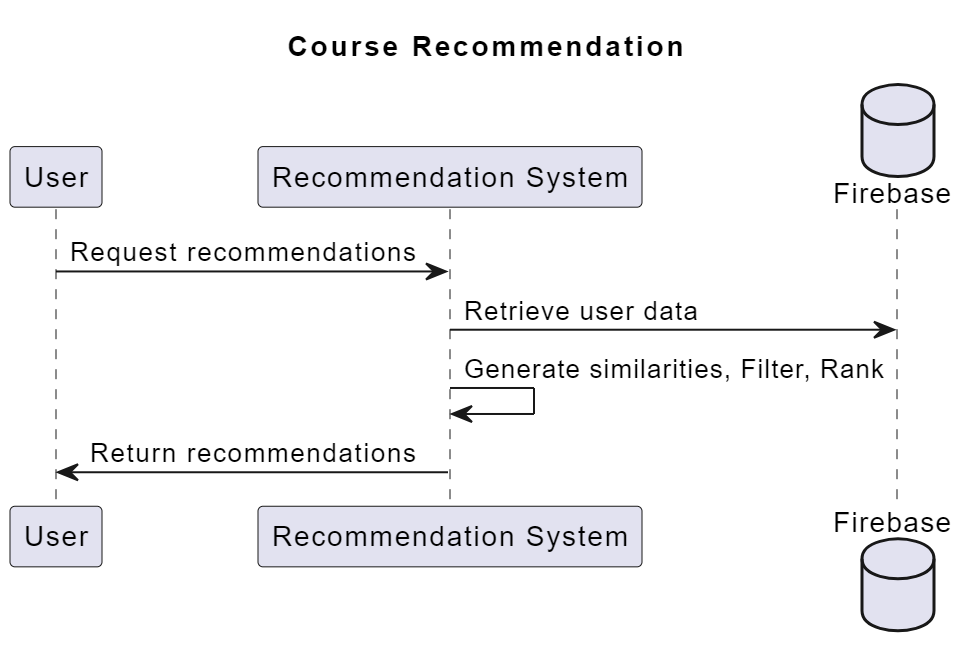
\includegraphics[width=0.8\textwidth]{3/course.png}
\caption{Course Recommendation Function}
\label{fig:course_recommendation}
\end{figure}

\section{Job Skillset Recommendation}

The Job Skillset Recommendation Module analyzes user input and matches it with relevant job skillsets from the dataset. This involves employing recommendation algorithms, such as cosine similarity measures, to identify similarities between user preferences and required job skills.

\begin{figure}[h]
\centering
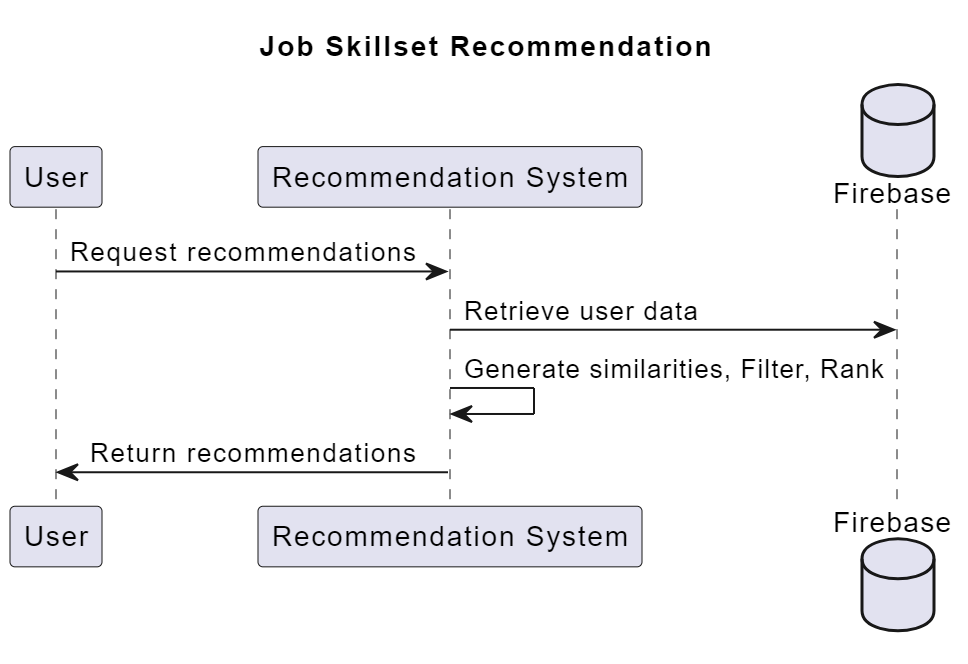
\includegraphics[width=0.8\textwidth]{3/skillset.png}
\caption{Job Skillset Recommendation Function}
\label{fig:job_skillset_recommendation}
\end{figure}

\section{Database Management}

The Database Management Module is responsible for storing and managing the dataset of courses and job skillsets. It ensures data integrity, facilitates efficient retrieval of information, and supports the updating of recommendations based on new data.

\begin{figure}[h]
\centering
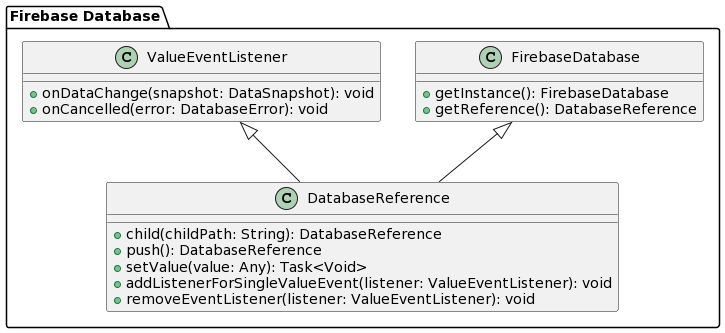
\includegraphics[width=0.8\textwidth]{3/database.png}
\caption{Database Architecture}
\label{fig:database_architecture}
\end{figure}

\section{Web Crawler}

The Web Crawler Module is responsible for gathering data from external sources to enrich the recommendation system. It automatically extracts information relevant to courses and job skillsets from websites, forums, or other online platforms. This data includes updated course listings, job postings, and industry trends.

\begin{figure}[h]
\centering
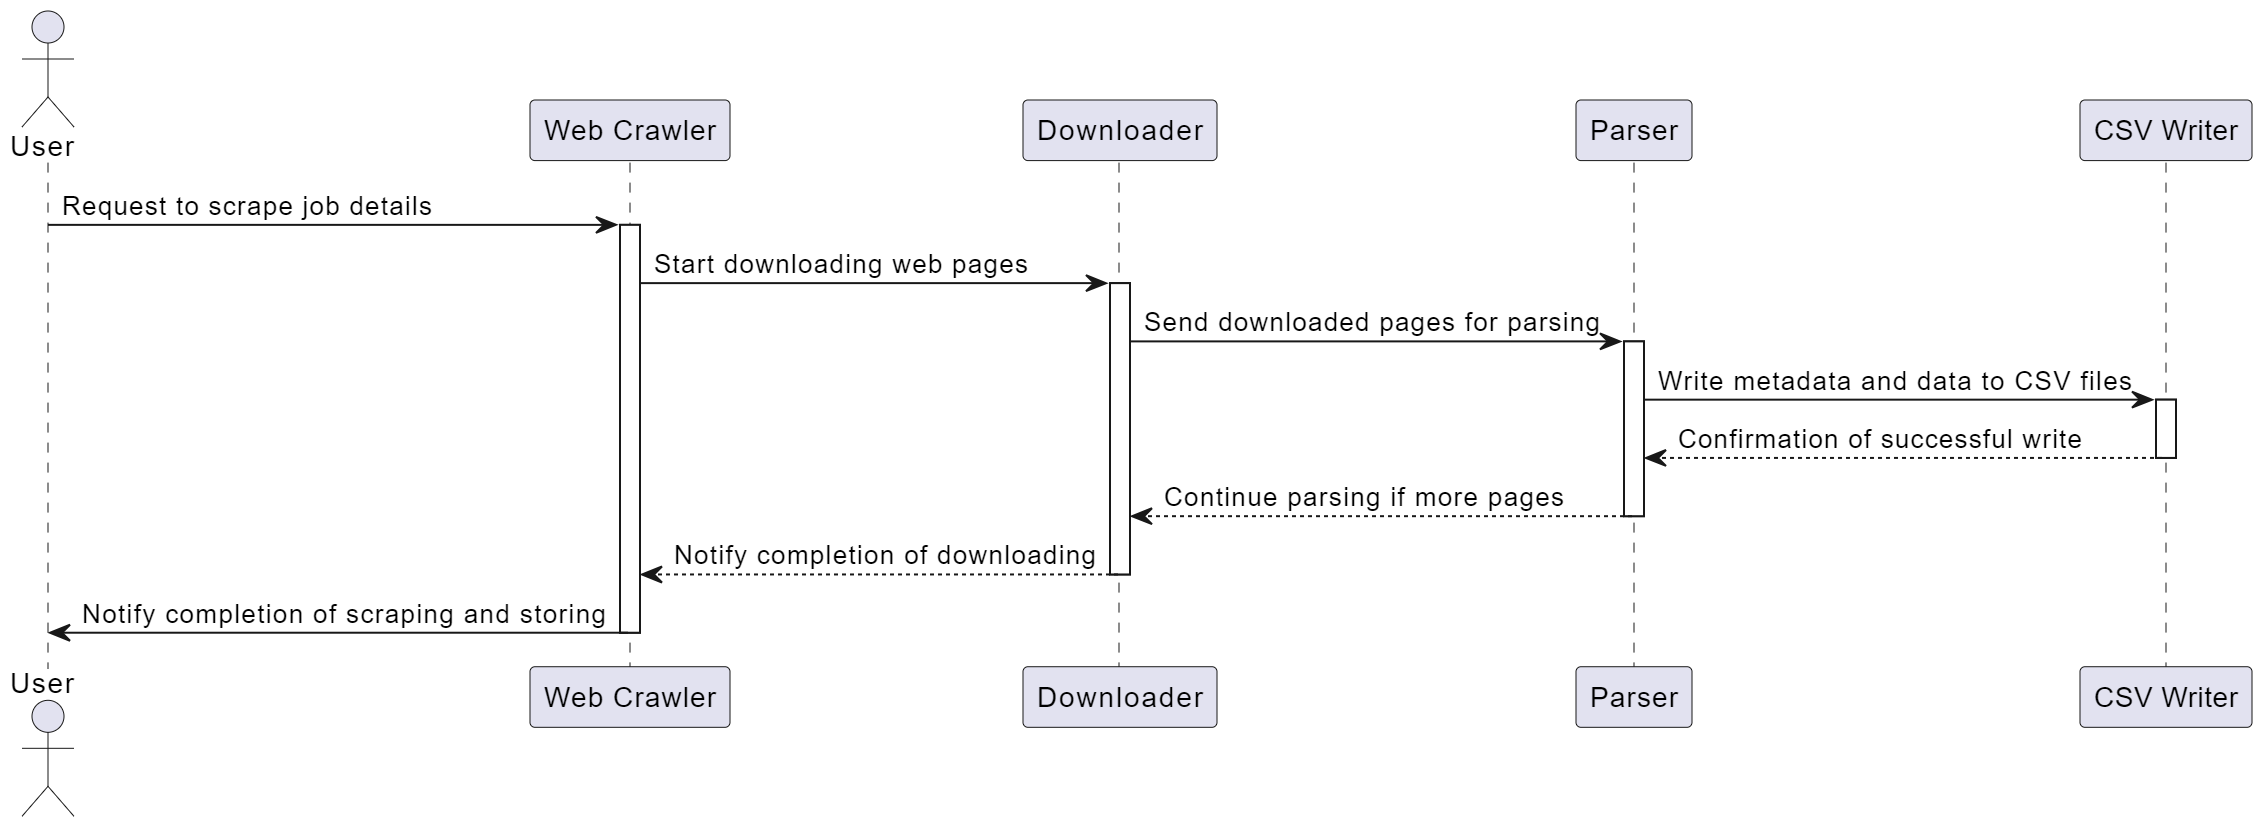
\includegraphics[width=0.8\textwidth]{3/webcrawler.png}
\caption{System Architecture for Web Crawler}
\label{fig:web_crawler}
\end{figure}